\section{\textbf{Joint-Output AGI-Former}}

The joint-output architecture extends AGI-Former from parallel outputs conditioned separately by each modality to one coordinated thought--action sequence. Its defining operation is not concatenation alone, but the placement of concatenation after each modality has been conditioned on the current causal state. Each branch first selects and transforms the evidence relevant to the pending decision. The selected representations are then assembled into a multimodal memory that conditions a final Unified Cross-MHA decoder.

Figure~\ref{fig:agi_former_joint} presents this organization. The modality encoders and causal Unified MHA encoder-in-decoder retain the roles defined in Sections~III and IV. Unlike the disjoint architecture, however, the outputs of the first-stage Unified X-MHA decoders are intermediate action-conditioned representations rather than independently executable commands. Concatenation combines these representations, and a second Unified X-MHA decoder generates the joint output tokens.

\begin{figure*}[t]
    \centering
    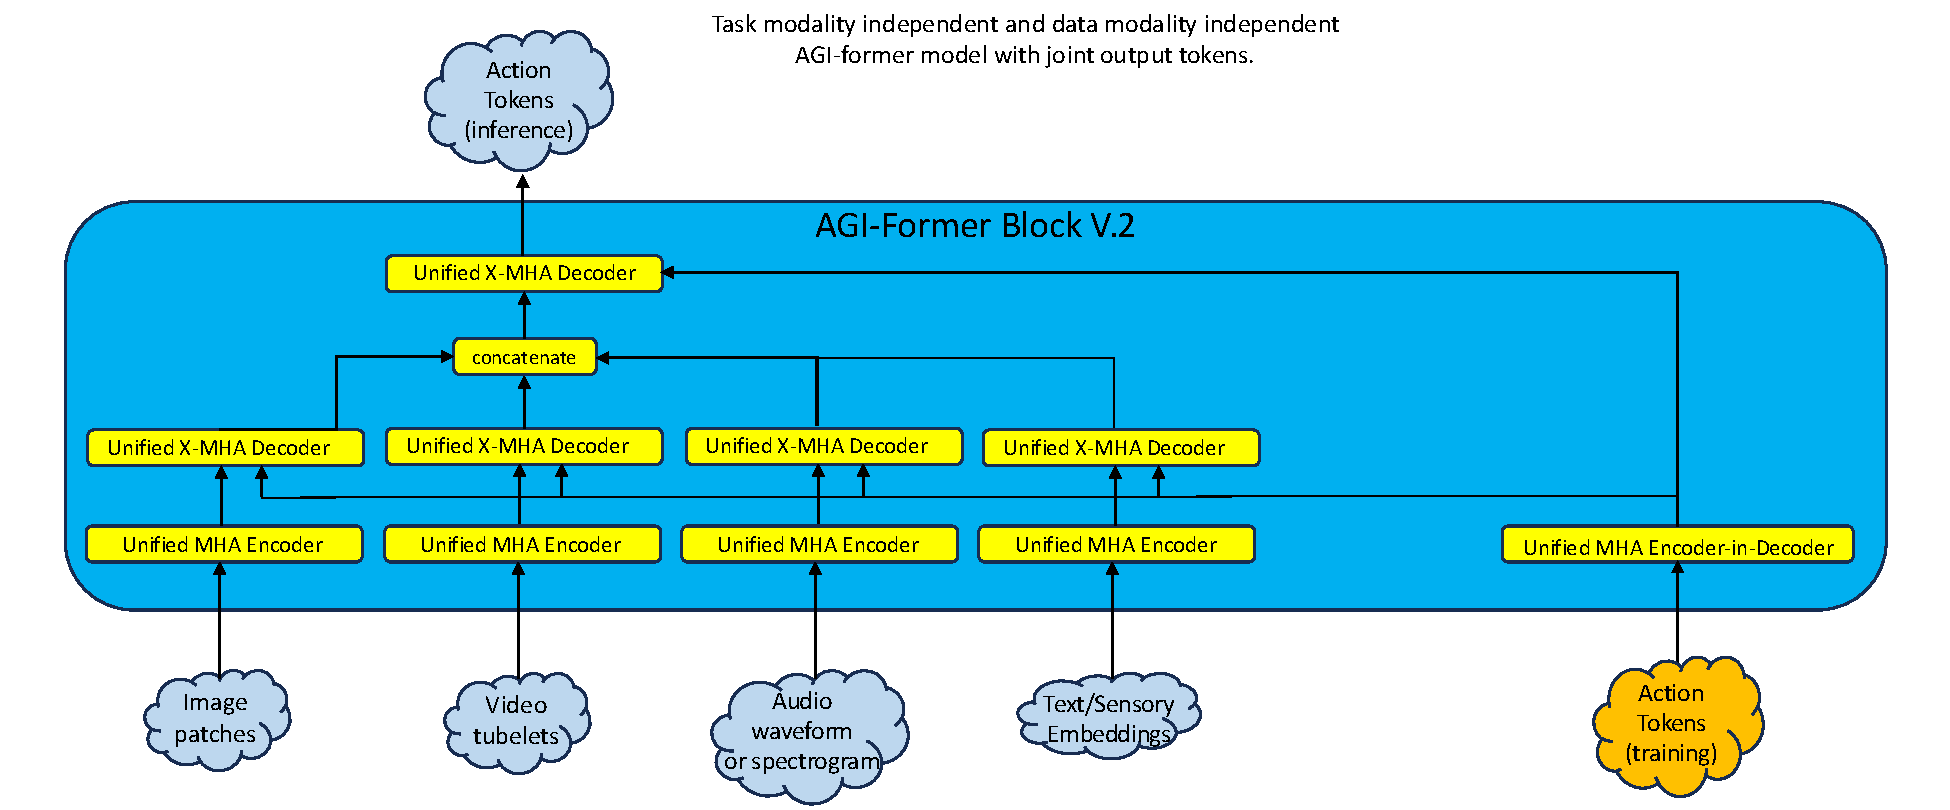
\includegraphics[width=\textwidth]{Figures/fig3.pdf}
    \caption{Joint-output AGI-Former. Each modality is encoded independently and conditioned on the shared causal thought--action state through a first-stage Unified Cross-MHA decoder. The conditioned representations are concatenated into a multimodal memory. A final Unified Cross-MHA decoder attends to that memory from the same causal state and generates one coordinated action-token sequence.}
    \label{fig:agi_former_joint}
\end{figure*}

\subsection{\textbf{First-Stage Action-Conditioned Representations}}

For each available modality $m\in\mathcal{M}$, the Unified MHA encoder produces $H_t^{(m)}$ as defined in Eq.~\eqref{eq:disjoint_modality_encoder}. The causal Unified MHA encoder-in-decoder produces $S_t$ from ground-truth history during training or generated history during inference according to Eq.~\eqref{eq:disjoint_action_state}. A first-stage Unified X-MHA decoder then computes

\begin{equation}
\begin{aligned}
    R_t^{(m)}
    &= \operatorname{UXMHA}^{(1)}_{m}\!\left(
       S_t,H_t^{(m)};\theta_{C_m}
       \right)
     \in\mathbb{R}^{L_t\times d},\\
    &\hspace{7.2cm}
       m\in\mathcal{M},\;r_t^{(m)}=1.
\end{aligned}
\label{eq:joint_conditioned_modality}
\end{equation}

The shared query length $L_t$ aligns every $R_t^{(m)}$ with the current thought--action state while permitting the encoded memories $H_t^{(m)}$ to retain different lengths. Thus, an image branch may attend over spatial patches, a video branch over tubelets, an audio branch over temporal or spectrogram tokens, and a language branch over text or sensor embeddings without requiring equal input geometry.

The intermediate representation $R_t^{(m)}$ is not interpreted as a complete action from modality $m$. It represents the evidence selected from that modality in response to the current causal state. This distinction separates joint AGI-Former from a voting or post-hoc aggregation system: the branches produce decision-conditioned evidence, not competing final decisions.

\subsection{\textbf{Action-Conditioned Late Fusion}}

Let $e_m\in\mathbb{R}^{d}$ be a learned modality-identity embedding broadcast across the positions of branch $m$. The active branch representations are concatenated along the token axis:

\begin{equation}
\begin{aligned}
    F_t
    &= \mathop{\operatorname{Concat}}_{m\in\mathcal{M}:r_t^{(m)}=1}
       \left(R_t^{(m)}+\mathbf{1}_{L_t}e_m^{\top}\right),\\
    F_t
    &\in\mathbb{R}^{L_t|\mathcal{M}_t|\times d},\\
    \mathcal{M}_t
    &= \left\{m\in\mathcal{M}:r_t^{(m)}=1\right\}.
\end{aligned}
\label{eq:joint_concatenation}
\end{equation}

The modality embeddings preserve source identity after concatenation. Positional or temporal embeddings remain attached to the tokens within each branch. A fusion mask $B_t$ identifies valid positions when branch sequences are padded or batched:

\begin{equation}
\begin{aligned}
    B_t[i]
    &=
    \begin{cases}
        0,       & \text{if }F_t[i,:]\text{ is valid},\\
        -\infty, & \text{if }F_t[i,:]\text{ is padding}.
    \end{cases}
\end{aligned}
\label{eq:joint_fusion_mask}
\end{equation}

Because each $R_t^{(m)}$ is already conditioned on $S_t$, Eq.~\eqref{eq:joint_concatenation} implements action-conditioned late fusion. An early-fusion alternative would concatenate $H_t^{(m)}$ before any branch-specific interaction with the causal state. That alternative is a valid ablation, but it asks a single fusion stage to discover both within-modality relevance and cross-modal coordination simultaneously.

\subsection{\textbf{Final Unified Cross-MHA Synthesis}}

The final Unified X-MHA decoder uses the causal state as its decoding stream and the concatenated representation $F_t$ as multimodal memory:

\begin{equation}
\begin{aligned}
    J_t
    &= \operatorname{UXMHA}^{(2)}\!\left(
       S_t,F_t,B_t;\theta_J
       \right)
     \in\mathbb{R}^{L_t\times d}.
\end{aligned}
\label{eq:joint_final_decoder}
\end{equation}

At final decoder layer $\ell$, the corresponding residual computation is

\begin{equation}
\begin{aligned}
    U_{t,\ell}
    &= \operatorname{LN}\!\left(
       J_{t,\ell}+
       \operatorname{UXMHA}^{(2)}_{\ell}\!\left(
       J_{t,\ell},F_t,B_t
       \right)
       \right),\\
    J_{t,\ell+1}
    &= \operatorname{LN}\!\left(
       U_{t,\ell}+
       \operatorname{FFN}^{(2)}_{\ell}\!\left(U_{t,\ell}\right)
       \right).
\end{aligned}
\label{eq:joint_final_layer}
\end{equation}

This second attention stage can compare evidence selected independently from different modalities. It may, for example, align an observed object with a spoken instruction, reconcile motion in video with a sound event, or suppress a text hypothesis contradicted by current sensory evidence. The output remains conditioned on $S_t$, preserving continuity with prior decisions rather than treating the fused memory as an isolated multimodal sample.

\subsection{\textbf{Joint Output Space}}

Let $\mathcal{V}_{J}$ be the vocabulary of the joint output stream. It may include natural-language tokens, internal control tokens, tool identifiers, action-type markers, quantized control values, and termination symbols. The next-token distribution is

\begin{equation}
\begin{aligned}
    P_t^{J}
    &= \operatorname{softmax}\!\left(
       J_tW_O^{J}+b_O^{J}
       \right),\\
    \widehat{y}_{t,j}^{J}
    &\sim P_t^{J}[j,:],
    &&j=1,\ldots,L_t.
\end{aligned}
\label{eq:joint_output_head}
\end{equation}

An output grammar or typed-token mask $G_{t,j}\in\{0,-\infty\}^{|\mathcal{V}_J|}$ can prohibit syntactically or physically invalid tokens:

\begin{equation}
\begin{aligned}
    P_{t,j}^{J}
    &= \operatorname{softmax}\!\left(
       z_{t,j}^{J}W_O^{J}+b_O^{J}+G_{t,j}
       \right).
\end{aligned}
\label{eq:joint_typed_mask}
\end{equation}

The mask constrains output validity but does not determine which valid action should be selected. That decision remains learned from the joint representation.

\subsection{\textbf{Training Objective}}

For teacher-forced training, the principal joint loss is the negative log-likelihood of the target output sequence:

\begin{equation}
\begin{aligned}
    \mathcal{L}_{J}
    &= -\sum_{t=1}^{T}
       \sum_{j=1}^{L_t}
       \log P_{t,j}^{J}\!\left[y_{t,j}^{J}\right].
\end{aligned}
\label{eq:joint_primary_loss}
\end{equation}

A model trained only through $\mathcal{L}_{J}$ could underuse one or more branches when another modality predicts the target sufficiently well. Optional auxiliary losses can preserve branch-level grounding:

\begin{equation}
\begin{aligned}
    \mathcal{L}_{\mathrm{joint}}
    &= \mathcal{L}_{J}
       +\sum_{m\in\mathcal{M}}
        \alpha_m\mathcal{L}_{\mathrm{aux}}^{(m)}
       +\beta\mathcal{L}_{\mathrm{align}}
       +\gamma\mathcal{L}_{\mathrm{reg}},\\
    \alpha_m,\beta,\gamma&\geq0.
\end{aligned}
\label{eq:joint_total_loss}
\end{equation}

Here, $\mathcal{L}_{\mathrm{aux}}^{(m)}$ may predict branch-relevant targets, $\mathcal{L}_{\mathrm{align}}$ may encourage correspondence across synchronized modalities, and $\mathcal{L}_{\mathrm{reg}}$ may include modality-dropout or attention-entropy regularization. These terms are optional and must be ablated; the defining joint architecture is given by Eqs.~\eqref{eq:joint_conditioned_modality}--\eqref{eq:joint_final_decoder}.

During training, modality dropout samples subsets $\mathcal{M}_t\subseteq\mathcal{M}$ so that the final decoder cannot assume that every stream is always present. For a retention probability $p_m$,

\begin{equation}
\begin{aligned}
    r_t^{(m)}&\sim\operatorname{Bernoulli}(p_m),\\
    \mathcal{M}_t&=\left\{m:r_t^{(m)}=1\right\},
    \qquad
    |\mathcal{M}_t|\geq1.
\end{aligned}
\label{eq:joint_modality_dropout}
\end{equation}

This procedure trains one parameterization over variable modality sets and supports direct testing of robustness to missing or corrupted inputs.

\subsection{\textbf{Autoregressive Inference}}

At inference step $j$, the model recomputes or caches the causal state, conditions each available modality, constructs $F_t$, and samples or selects the next joint token. The recurrence is

\begin{equation}
\begin{aligned}
    S_{t,j}
    &= \operatorname{UMHAED}\!\left(
       \widehat{Y}_{<t},\widehat{y}_{t,<j}^{J}
       \right),\\
    R_{t,j}^{(m)}
    &= \operatorname{UXMHA}^{(1)}_m\!\left(
       S_{t,j},H_t^{(m)}
       \right),\\
    F_{t,j}
    &= \operatorname{Concat}_{m\in\mathcal{M}_t}
       \left(R_{t,j}^{(m)}+e_m\right),\\
    \widehat{y}_{t,j}^{J}
    &\sim p_{\theta}\!\left(
       \cdot\mid S_{t,j},F_{t,j}
       \right).
\end{aligned}
\label{eq:joint_inference}
\end{equation}

Caching encoder outputs and past decoder states avoids repeating computations that do not change within the decision step. When new sensor measurements arrive during generation, only the affected branch and downstream fusion computations need to be refreshed.

\subsection{\textbf{Complexity and Architectural Tradeoffs}}

Let $L$ denote the causal-state length and $N_m$ the encoded length of modality $m$. Ignoring encoder-internal costs and constants associated with attention heads, first-stage cross-attention requires

\begin{equation}
\begin{aligned}
    \mathcal{C}_{1}
    &= \mathcal{O}\!\left(
       dL\sum_{m\in\mathcal{M}_t}N_m
       \right).
\end{aligned}
\label{eq:joint_stage_one_complexity}
\end{equation}

Concatenation produces $L|\mathcal{M}_t|$ memory tokens. The final cross attention therefore requires

\begin{equation}
\begin{aligned}
    \mathcal{C}_{2}
    &= \mathcal{O}\!\left(
       dL^2|\mathcal{M}_t|
       \right).
\end{aligned}
\label{eq:joint_stage_two_complexity}
\end{equation}

The second stage is the principal additional cost relative to disjoint branches. Token pooling, learned compression, sparse attention, or branch selection may reduce this cost, but each changes the information available for joint synthesis and must therefore be evaluated rather than assumed equivalent.

The joint architecture resolves the principal limitation of the disjoint design: all active modalities influence one learned output before execution. It also introduces new risks. A dominant modality may suppress weaker streams; concatenation increases memory; conflicting evidence may destabilize attention; and one shared output vocabulary can become difficult to balance across heterogeneous action types. The disjoint and joint models should therefore be treated as alternative hypotheses whose relative value depends on the task, output semantics, training data, and deployment constraints. Section~VI develops the experimental protocol needed to compare them.
